\section{User Study}

% \subsection{Foreword}
% By combining the plug-and-play mechanism of breadboards and the rapid routing of PCP, whether the combination of the benefits results in faster prototyping times is of interest. Therefore, both a breadboard and PCP should be evaluated as a basis of comparison to \papertitle.

%However, a decision to remove printable circuits as a member of the three prototyping tools was made. This is a result of two aspects, reliability and functionality. 
%熬夜
%寫,太強了!!!! 你這邊可以再說一次你覺得怎麼樣寫比較好嗎?
%就是,我們參考並結合了麵包板的插拔機制以及PCP的快速產生線路的機制。
%我們想要知道兩者的結合是否可以產生更快的速度,因此我們就必須去個別比較過去這兩個工具看看有沒有真的比較快,這樣可以嗎?XD 

%歐歐我想起來了 感謝~ (good job, but please go to bed early!! Not healthy to stay up this late! You need health to work in the following days~!) ok, will finish up quickly here :D

% The first reason was due to the unreliable nature of previous works in this area.
% In the beginning, we followed the convention laid out by \cite{Instant_Inkjet_Circuits}.
% Despite claiming to be an effective method, the 3M conductive tape suggested by \cite{Instant_Inkjet_Circuits} was proven to be a liability in component connection by \cite{Circuit_Stickers} and our 3-person pilot study. Enormous pressure and heat had to be applied to obtain a reliable connection between a component and printed circuit.

% Therefore, we modified our components to use IC sockets for an uniform 90 degree contact area. Thus, in our original study, users were given modified components in the printable circuit section.
% However, the functionality of printable circuits was called into question. The high level of component customization required (e.g. Circuit Sticker) to allow for complete functionality or faster prototyping results in the loss of rapidness in prototyping.

% However, \cite{Circuit_Stickers} suggested that the 3M conductive tape is a liability in component connection due to small contact areas between a component pin and the tape. To verify this, we launched a 5-person pilot study asking participants to attach a seven segment display via 3M conductive tape to PCP on which lies a suitable ink pattern to place a seven segment display resembling Figure 7b in \cite{Instant_Inkjet_Circuits}. We concluded that averagely 18\% of the pins are electrically connected to the conductive ink through the 3M tape. Although \cite{Circuit_Stickers} proposes a solution by expanding contact areas, great efforts with high level of component customization to allow for reliable connections, complete functionality, and faster prototyping results in the loss of rapidness in prototyping. Thus, we remove PCP from our evaluation.

% However, \cite{Circuit_Stickers} suggests that the 3M conductive tape has poor reliability in component connection. To verify this, we imitate Figure 7b in \cite{Instant_Inkjet_Circuits} and conclude that only 18\% of the pins are electrically connected to the conductive ink through the 3M tape. Thus, we remove PCP from our evaluation.

%In our pilot study, we found that the unreliable nature of printable circuits resulted in the lack of functionality in our implementation... Therefore...

% Combining the two critical flaws mentioned above, we decided to exclude printable circuits from the tested tools in our study.

\subsection{Chosen Circuits}

To evaluate the convenience and modification ability of breadboard and \papertitle, we choose to construct a series of circuits with different difficulty levels of LEDs along with an Arduino Mega board (\autoref{fig:Chosen_Circuits}). Each circuit builds off the previous as if building a prototype part by part.
%把下面的放進圖片敘述
% The first circuit consists of a temperature sensor (LM35) and a LED that turns on as the temperature rises 3\textcelsius. Without changing the first circuit, a RGB LED is then added to signify the range that the temperature is in. The RGB LED will change smoothly from aqua to green to red every increment of 3\textcelsius. Lastly, a four-digit seven segment is added to display the temperature reading in Celsius.

\begin{figure}[h]
  \begin{center}
  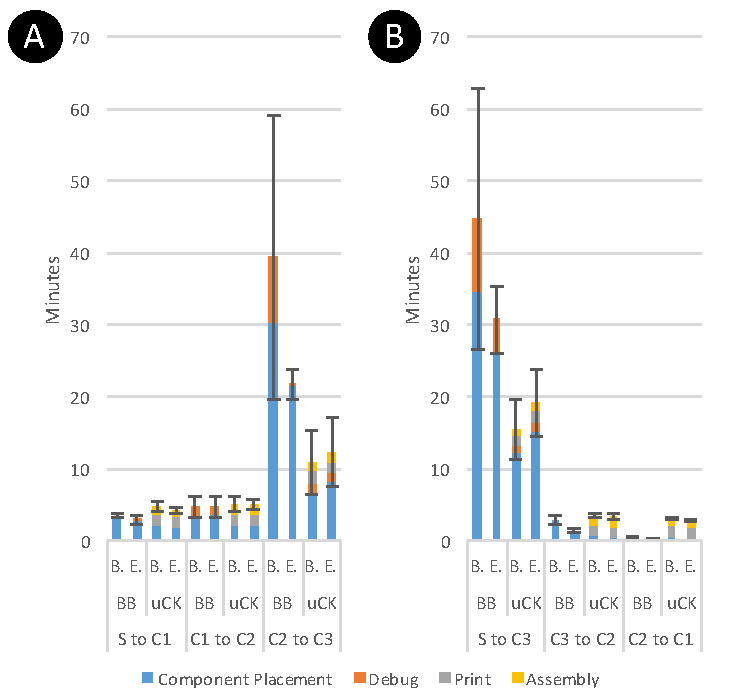
\includegraphics[width=1\columnwidth]{figures/Circuit_Construction_Duration_v15.pdf}
  \caption{In the following figures C1 is short for \textit{Circuit 1} and so forth. S means the empty scratch state. BB stands for breadboard and uCK is brief for \papertitle. Lastly, B is short for beginner and E is short for expert. (A) is the average completion time in additive sequence divided into beginner and expert. (B) is the average completion time in subtractive sequence divided into beginner and expert.}
  \label{fig:Circuit_Construction_Duration}
  \end{center}
\end{figure}

\subsection{Procedure}

16 participants (5 females, mean age 22.9) were recruited from departments of electrical engineering and computer science engineering. Half are beginners who have little or no prototyping experiences using a breadboard with less than 10 projects, and the other half vice versa.

Participants were asked to complete the 3 circuits with full functionality in either an additive or subtractive circuit construction order starting from namely \textit{Circuit 1} to \textit{3} or \textit{3} to \textit{1}, respectively, by using the 2 tools in random order. In addition to circuit components, participants were given full information for circuit construction on a monitor including Fritzing schematics, circuit schematics, and datasheet. Participants were also allowed to operate a computer for searching additional information or adjusting the monitor display view.

Participants do not need to remove components from the previous circuit during additive circuit construction but must remove unnecessary components during subtractive circuit construction.

Lastly, participants were interviewed to express their opinions regarding the convenience and modification ability of the two tools.

% \subsubsection{Pre-evaluation}
% Users were first asked to answer a questionnaire in order to obtain basic information regarding age and gender. Then, users were asked how many times they have used breadboards in the past, and if they had any experience at all they were asked the source of their exposure and the most difficult circuit they have prototyped. To conclude the pre-evaluation, users were asked they have tried other prototyping tools and if so, which ones.

% Users were asked to fill a questionnaire including prototyping experiences using a breadboard to obtain basic background information.

% \subsubsection{Environment Setup}
% Our study environment consists of three stages for each prototyping tool under evaluation. At each station, parts and Arduino Mega boards are all laid out for users to use. Users are shown schematics on a monitor in order to assist in completion of the tasks and are recorded for the entirety of the study.

% \subsubsection{"Blink"}
% We prepared a warm-up exercise obtained from the Official Arduino Website for non-experts to practice.
% The exercise, called "Blink", involves connecting a LED and turning it on and off every second by toggling the HIGH LOW of the LED.
% This warm-up activity was used before the start of every prototyping tool session.

% We prepared a warm-up exercise called "Blink" from the Official Arduino Website for beginners to practice on each prototyping tool session.

% \subsubsection{Prototyping Tools}
% Our evaluation encompasses breadboard, and lastly \papertitle. For every tool, users are asked to complete the chosen circuits. However, we choose to randomize the order in which users tried each tool, because REASON. Furthermore, during the chosen circuits part, some users are asked to complete the most complicated circuit, then work in reverse back to a simple LED with temperature sensor. We determined that this method would help REASON. 

% \subsubsection{Post-Evaluation}
% After completion of the two tools, users were given a questionnaire that asked them to rank the convenience and modification ability of the two tools. Users were also given an opportunity to comment with any thoughts that they had during the study.